\documentclass[12pt]{article}
\usepackage{amscd,amssymb,amsthm,amsxtra,exscale,latexsym,verbatim,paralist}
\usepackage{mathrsfs}
\usepackage[T1]{fontenc}
\usepackage{newtxmath,newtxtext}
\usepackage[left = 2.5cm, top = 3cm, bottom = 3cm, right = 2.5cm]{geometry}

\usepackage{hyperref}
\usepackage{tikz}

\newcommand{\XB}{\color{black}}
\newcommand{\XBB}{\color{blue}}
\newcommand{\XV}{\color{violet}}
\newcommand{\XR}{\color{red}}

\pagestyle{empty} 
\setlength{\parindent}{0pt} 
\setlength{\parskip}{\baselineskip}

\theoremstyle{plain}
\newtheorem{ex}{Exercise}

\renewcommand{\proofname}{Solution}

\begin{document}

\title{\textbf{MTH385}: History of Mathematics - Homework \#2}
\date{}
\author{\XV\textit{\large{\href{https://github.com/casonk}{Cason Konzer}}}\XB}

\maketitle

\hrulefill

\newpage

%%%%%%%%%     #1     %%%%%%%%%%%%%%%%%%%%%%%%%%%%%%%%%%%%%%%%%%%%%%%%%%%%%%%%%%%%%%%%%%%%%%%%%
\XBB\hrulefill\XB \\
\begin{ex} [1.5.2]
  Show that the square of $2q+1$ is in fact of the form $4s+1$, and hence explain why every integer square leaves remainder $0$ or $1$ on division by $4$.
\end{ex}
\XBB\hrulefill\XB \\
\begin{proof}
  \ \\
  Note: $\%$ is used as the modulus operator.
  \begin{itemize}
    \item Taking the square of $2q+1$ we have the following \dots
    \subitem $ (2q+1)^{2} = 4q^{2} + 4q + 1 = 4(q^{2} + q) + 1$
    \item Letting $ s = q^{2} + q $ we have the form $4s+1$.
    \item Considering $ q $ integer, we have two cases to equate.
    \item For $ q $ $even$ we have $ q = 2k$, $k \in \mathbb{Z} $.
    \subitem $ q^{2} = (2k)^{2} = 4k^{2} $.
    \subitem $ q^{2} \ \% \ 4 = 4k^{2} \ \% \ 4 = 0 $.
    \item For $ q $ $odd$ we have $ q = 2k+1$, $k \in \mathbb{Z} $.
    \subitem $ q^{2} = (2k+1)^{2} = 4k^{2} + 4k + 1 = 4(k^{2} + k) + 1 $.
    \subitem $ q^{2} \ \% \ 4 = (4(k^{2} + k) + 1) \ \% \ 4 = ((4(k^{2}+k) \ \% \ {4})+(1 \ \% \ {4})) \ \% \ {4} = (0+1) \ \% \ {4} = 1 $.
    \item Hence every integer square leaves remainder $0$ or $1$ on division by $4$.
  \end{itemize}
\end{proof}

\newpage
%%%%%%%%%     #2     %%%%%%%%%%%%%%%%%%%%%%%%%%%%%%%%%%%%%%%%%%%%%%%%%%%%%%%%%%%%%%%%%%%%%%%%%
\XBB\hrulefill\XB \\
\begin{ex} [2.1.1]
  Explain how Common Notions~1 and 4 may be interpreted as the transitive and reflexive properties. Note that the natural way to write Common Notion 1 symbolically is slightly different from the statement of transitivity above.
\end{ex}
\XBB\hrulefill\XB \\
\begin{proof}
  \ \\
  \begin{itemize}
    \item \textit{Common Notions} $1$ says : Things which are equal to the same thing are also equal to one another.
    \subitem From this notion we will take two things equal to the same thing, $ a = b $ and $ c = b $.
    \subitem It can be seen that from the notion as both $ a $ and $ c $ are equal to the same thing, $ b $, then $ a $ and $ c $ are equal to one another. 
    \subitem This can be interpreted as the \textit{transitive} property: $ a \cong b, \ b \cong c \Rightarrow a \cong c $.
    \item \textit{Common Notions} $4$ says : Things which coincide with one another are equal to one another.
    \subitem Having two things coincide can be thought of as two points taking the same coordinates, or two lines/angles laid on oneanother. 
    \subitem We conclude from this notion that these two objects are equal to one another, of which they are then the same base object. 
    \subitem Taking the points as an example, we have $ p_1 \cong p_2 \cong p $ and $ p_2 \cong p_1 \cong p $ where $ p $ is the base object.
    \subitem The reflexive property follows nicely as $ p \cong  p $.
  \end{itemize}
\end{proof}

\newpage
%%%%%%%%%     #3     %%%%%%%%%%%%%%%%%%%%%%%%%%%%%%%%%%%%%%%%%%%%%%%%%%%%%%%%%%%%%%%%%%%%%%%%%
\XBB\hrulefill\XB \\
\begin{ex} [2.1.2]
  Show that the symmetric property follows from Euclid's Common Notions~1 and 4.
\end{ex}
\XBB\hrulefill\XB \\
\begin{proof}
  \ \\
  \begin{itemize}
    \item From above we have $ a \cong b $ and $ a \cong a $
    \subitem By the \textit{reflexive} property, $ a \cong a \cong b $
    \subitem As $ a \cong b $, $ a \cong b \cong a \cong b $
    \subitem Since $ b \cong b $ and $ a \cong a $, we see that $ b \cong b \cong a \cong a $
    \subitem It then follows that $ b \cong a $.
    \item We have thus shown that the \textit{symmetric} property, $ a \cong b \Rightarrow b \cong a $, follows as as result of \textit{Euclid's Common Notions} $1$ and $4$.
  \end{itemize}
\end{proof}

\newpage
%%%%%%%%%     #4     %%%%%%%%%%%%%%%%%%%%%%%%%%%%%%%%%%%%%%%%%%%%%%%%%%%%%%%%%%%%%%%%%%%%%%%%%
\XBB\hrulefill\XB \\
\begin{ex} [2.2.1]
  Show that $\displaystyle \frac{\text{circumradius}}{\text{inradius}}=\sqrt{3}$ for both the cube and the octahedron.
\end{ex}
\XBB\hrulefill\XB \\
\begin{proof}
  \ \\
  Consider the following figure. \\
  \begin{center}
    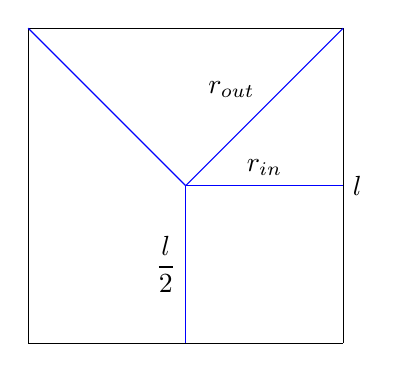
\begin{tikzpicture}
      \draw (-2,-2) -- (-2,2);
      \draw (-2,-2) -- (2,-2);
      \draw (2,2) -- (-2,2);
      \draw (2,2) -- (2,-2);
      \draw [blue] (0,0) -- (2,0);
      \draw [blue] (0,0) -- (-2,2);
      \draw [blue] (0,0) -- (2,2);
      \draw [blue] (0,0) -- (0,-2);
      \node [left] at (0,-1) {$\displaystyle \frac{l}{2}$};
      \node [above] at (1,0) {$r_{in}$};
      \node [above left] at (1,1) {$r_{out}$};
      \node [right] at (2,0) {$l$};
    \end{tikzpicture}
  \end{center}
  \begin{itemize}
    \item We will utilize the cross sectional square of the cube, with side length $l$, shown above. 
    \subitem From basic geometry we can see that  $\displaystyle r_{in} = \frac{l}{2}$.
    \item We can also see that $r_{out}$ is the hypotenuse of the tiangle with base and height $r_{in}$.
    \subitem From the Pythagorean Theorem, $r_{out}^{2} = r_{in}^{2} + r_{in}^{2} $
    \subitem Thus $\displaystyle r_{out}^{2} = \frac{l^{2}}{4} + \frac{l^{2}}{4} = \frac{l^{2}}{2} $
    \subitem We can now see that $\displaystyle r_{out} = \frac{l}{\sqrt{2}}$
    \item Consider the unit cube as a means to find the ratio between $r_{circum}$ and $r_{out}$.
    \item $r_{out}$ is the distance from $(0,0,0)$ to $(1,1,0)$.
    \subitem This distance $d_{out}$ is simply $\sqrt{(1-0)^2 + (1-0)^2 + (0-0)^2} = \sqrt{2} $.
    \item $r_{circum}$ is the distance from $(0,0,0)$ to $(1,1,1)$.
    \subitem This distance $d_{circum}$ is simply $\sqrt{(1-0)^2 + (1-0)^2 + (1-0)^2} = \sqrt{3} $.  
    \item Thus we have $\displaystyle d_{circum} = \frac{d_{out}\sqrt{3}}{\sqrt{2}}$.
    \subitem It follows that $\displaystyle r_{circum} = \frac{r_{out}\sqrt{3}}{\sqrt{2}} = \frac{\frac{l}{\sqrt{2}}\sqrt{3}}{\sqrt{2}} = \frac{l\sqrt{3}}{2} $.
    \item We now have acquired the relevant information to compute $\displaystyle \frac{\text{circumradius}}{\text{inradius}}$.
    \subitem $\displaystyle \frac{r_{circum}}{r_{in}} = \frac{\frac{l}{2}\sqrt{3}}{\frac{l}{2}} = \sqrt{3}$.
    \item We have show that $\displaystyle \frac{\text{circumradius}}{\text{inradius}}=\sqrt{3}$ for the cube.
  \end{itemize} 
  Consider next the following figure. \\
  \begin{center}
    \begin{tikzpicture}
      \draw (0,4) -- (-4,0);
      \draw (0,4) -- (4,0);
      \draw (0,-4) -- (-4,0);
      \draw (0,-4) -- (4,0);
      \draw [blue] (0,0) -- (0,4);
      \draw [blue] (0,0) -- (-4,0);
      \draw [blue] (0,0) -- (2,2);
      \draw [blue] (0,0) -- (2,-2);
      \node [below left] at (1,-1) {$\displaystyle \frac{l}{2}$};
      \node [left] at (0,2) {$r_{circum}$};
      \node [above right] at (2,2) {$l$};
    \end{tikzpicture}
  \end{center}
  \begin{itemize}
  \item We will utilize the cross sectional square of the octahedron, with side length $l$, shown above. 
  \item We can see that $l$ is the hypotenuse of the triangle with base and height $r_{circum}$.
  \subitem From the Pythagorean Theorem $ l^{2} = r_{circum}^{2} + r_{circum}^{2} = 2r_{circum}^{2} $.
  \subitem It follows that $\displaystyle r_{circum}^{2} = \frac{l^{2}}{2} $ and $\displaystyle r_{circum} = \frac{l}{\sqrt{2}} $.
  \item We know that $r_{in}$ can be constructed as the length of a line from the origin to the center of a face with respect to the octahedron.
  \item This line can be represented by the vector from $ (0,0,0) $ to $\displaystyle \bigl( \frac{r_{circum}}{3}, \frac{r_{circum}}{3}, \frac{r_{circum}}{3} \bigr) $.
  \item We thus have the length as the distance of this vector \dots
  \subitem $ \displaystyle d_{in} = \sqrt{ \bigl( 0-\frac{r_{circum}}{3} \bigr)^{2} + \bigl( 0-\frac{r_{circum}}{3} \bigr)^{2} + \bigl( 0-\frac{r_{circum}}{3} \bigr)^{2}} = \sqrt{3\bigl( \frac{r_{circum}}{3} \bigr)^{2}} = \frac{r_{circum}\sqrt{3}}{3} $.
  \subitem Thus we can see that $ \displaystyle r_{in} = \frac{r_{circum}}{\sqrt{3}} = \frac{l}{\sqrt{2}\sqrt{3}} $.
  \item We now have acquired the relevant information to compute $\displaystyle \frac{\text{circumradius}}{\text{inradius}}$.
  \subitem $\displaystyle \frac{r_{circum}}{r_{in}} = \frac{\frac{l}{\sqrt{2}}}{\frac{l}{\sqrt{2}\sqrt{3}}} = \frac{1}{\frac{1}{\sqrt{3}}} = \sqrt{3}$.
  \item We have show that $\displaystyle \frac{\text{circumradius}}{\text{inradius}}=\sqrt{3}$ for the octahedron.
\end{itemize}
\end{proof}

\newpage
%%%%%%%%%     #5     %%%%%%%%%%%%%%%%%%%%%%%%%%%%%%%%%%%%%%%%%%%%%%%%%%%%%%%%%%%%%%%%%%%%%%%%%
\XBB\hrulefill\XB \\
\begin{ex} [2.2.2]
  Check Pacioli's construction: use the Pythagorean theorem to show that $AB=BC=CA$ in Figure~2.2. (It may help to use the additional fact that $\tau=(1+\sqrt{5})/2$ satisfies $\tau^2=\tau+1$.)
\end{ex}
\XBB\hrulefill\XB \\
\begin{proof}
  \ \\
  Consider first \textit{Pacioli's} construction of the icosahedron. \\
  \begin{center}
    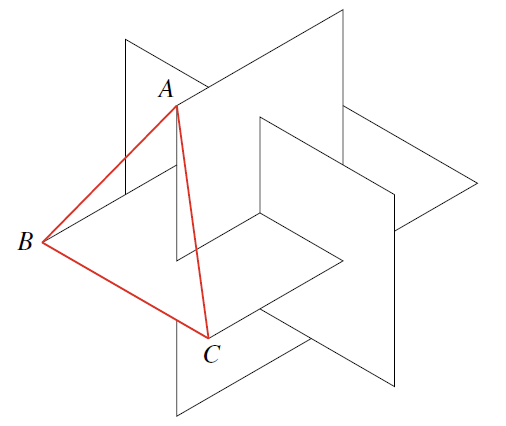
\includegraphics[width=0.48\textwidth]{icosahedron.png}
  \end{center}
  Consider the next \textit{golden rectangle}. \\
  \begin{center}
    \begin{tikzpicture}
      \draw (-3.23,-2) -- (-3.23,2);
      \draw (3.23,-2) -- (3.23,2);
      \draw (-3.23,-2) -- (3.23,-2);
      \draw (-3.23,2) -- (3.23,2);
      \node [above] at (0,2) {$\displaystyle \frac{1 + \sqrt{5}}{2} = \tau$};
      \node [right] at (3.23,0) {$1$};
    \end{tikzpicture}
  \end{center}
  \begin{itemize}
    \item We will let the $z$ coordinate of $B$ and $C$ be $0$ while the $y$ coordinant of $A$ be $0$.
    \item We can thus find the position of the points $A$, $B$, and $C$ in this coordinant system.
    \subitem $ \displaystyle A = \Bigl( \frac{1}{2}, 0, \frac{\tau}{2} \Bigr) \ , \ \ B = \Bigl( \frac{\tau}{2}, -\frac{1}{2}, 0 \Bigr) \ , \ \ C = \Bigl( \frac{\tau}{2}, \frac{1}{2}, 0 \Bigr) $.
    \item Thus we can now solve for $AB$, $BC$, and $CA$ by basic distance measures.
    \item $ \displaystyle AB = \sqrt{\Bigl( \frac{\tau}{2} - \frac{1}{2} \Bigr)^2 + \Bigl( -\frac{1}{2} - 0 \Bigr)^2 + \Bigl( 0 - \frac{\tau}{2} \Bigr)^2} = \sqrt{\Bigl( \frac{\tau - 1}{2} \Bigr)^2 + \Bigl( -\frac{1}{2} \Bigr)^2 + \Bigl( - \frac{\tau}{2} \Bigr)^2} $.
    \subitem $ \displaystyle = \sqrt{\Bigl( \frac{\tau^2 -2\tau + 1}{4} \Bigr) + \Bigl( \frac{1}{4} \Bigr) + \Bigl( \frac{\tau^2}{4} \Bigr)} = \sqrt{ \frac{\tau + 1 -2\tau + 1}{4} + \frac{1}{4} + \frac{\tau + 1}{4} } $.
    \subitem $ \displaystyle = \sqrt{ \frac{2 -\tau + 1 + \tau + 1}{4} } = \sqrt{\frac{4}{4}} = \sqrt{1} = 1 $.
    \item $ BC = 1 $, by the given length of the short side of the \textit{golden rectangle}.
    \item $ \displaystyle CA = \sqrt{\Bigl( \frac{1}{2} - \frac{\tau}{2} \Bigr)^2 + \Bigl( 0 - \frac{1}{2} \Bigr)^2 + \Bigl( \frac{\tau}{2} - 0 \Bigr)^2} = \sqrt{\Bigl( \frac{1 - \tau}{2} \Bigr)^2 + \Bigl( - \frac{1}{2} \Bigr)^2 + \Bigl( \frac{\tau}{2} \Bigr)^2} $.
    \subitem $ \displaystyle = \sqrt{\Bigl( \frac{\tau^2 -2\tau + 1}{4} \Bigr) + \Bigl( \frac{1}{4} \Bigr) + \Bigl( \frac{\tau^2}{4} \Bigr)} = \sqrt{ \frac{\tau + 1 -2\tau + 1}{4} + \frac{1}{4} + \frac{\tau + 1}{4} } $.
    \subitem $ \displaystyle = \sqrt{ \frac{2 -\tau + 1 + \tau + 1}{4} } = \sqrt{\frac{4}{4}} = \sqrt{1} = 1 $.
    \item We can now see that $AB=BC=CA=1$ and that \textit{Pacioli's} construction of the icosahedron holds.
  \end{itemize} 
\end{proof}

\end{document}

